\documentclass[thesis]{subfiles}

\begin{document}

\chapter{Methodology}
\label{methodology}

\section{Generalising Neural Networks and Decision Trees}
Here we explore the continuity of models between decision forests, with the objective of reducing the connectivity of deep neural networks trained with back-propagation, specifically convolutional neural networks, while retaining some of the efficiency and understanding which arise from the conditional computation in decision forests.

Towards this objective, we generalize neural networks and decision trees intuitively by using a new graphical notation for representing both. This notation isolates the differences between the two models, such that we can represent a hybrid model, \ie a \emph{Conditional Network}, compactly\footnote{This notation itself was created by Dr. Antonio Criminisi, and is not a contribution of this thesis. Some figures used with the permission of Dr. Antonio Criminisi/Microsoft Research.}.

\section{A New Graphical Notation}
The proposals we will make require a re-interpretation of existing classification models, that is neural networks and decision trees, but standard graphical diagrams for both of these models hides the implicit functional similarities on which we will build our models, and are instead connection-centric - focused on showing the connectivity of the models rather than the underlying data transformations. As such, before we are able to explain the concept of a conditional network, a new graphical language is proposed.

\subsection{Neural Networks}
\begin{figure}[htbp!] 
\centering
\begin{subfigure}[b]{0.45\textwidth}
   \centering
   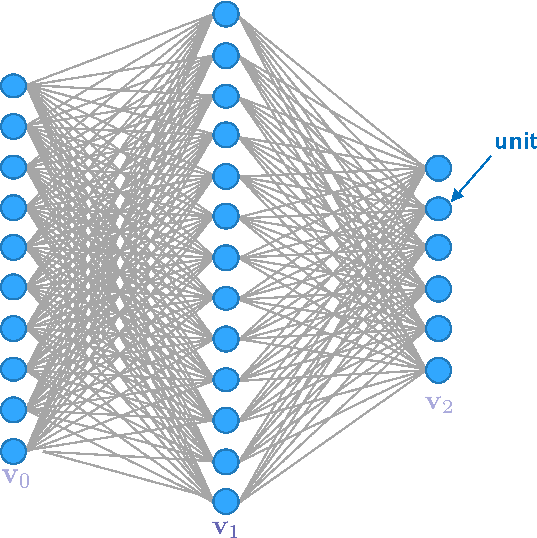
\includegraphics[width=\textwidth]{fullyconnected}
   \caption{Standard diagram of a neural network with one hidden layer.}
   \label{fig:oldnotation}
\end{subfigure}
~
\begin{subfigure}[b]{0.45\textwidth}
   \centering
   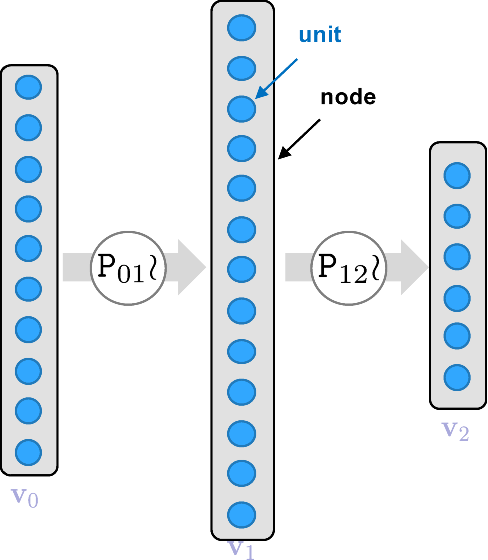
\includegraphics[width=0.9\textwidth]{newnotation}
   \caption{New notation showing transformation between layers explicitly.}
   \label{fig:newnotation}
\end{subfigure}
\caption[New graphical notation for a standard neural network with one hidden layer.]{The proposed compact graphical notation for neural networks. Non-linear transformations in a standard neural network with one hidden layer are indicated by the projection matrix $\mat P$ between the two layers, followed by a generic non-linearity, represented with the symbol $\wr$. Figures used with permission~\copyright Antonio Criminisi}
\label{fig:newGraphLanguage}
\end{figure}

The standard depiction of a neural network with one hidden layer is shown in Fig.~\ref{fig:oldnotation}, where each of the layers is fully connected, and these connecting weights are illustrated as lines between the neurons represented as circles. While this image illustrates the connectivity of the model, it assumes the function of the neurons themselves to be known or otherwise described. In Fig.~\ref{fig:newnotation}\ we use a different notation to show both connectivity and function of each layer, with the assumption that all nodes on a particular layer have the same function.

In this simple example of a fully-connected neural network, between layers $i$ and $j$, every node outputs the non-linear transformation, $\vec v_j = \sigma(\mat P \vec v_i)$, a composition of the non-linear function $\sigma$ (\eg a ReLU or sigmoid) and the projection of the input units with a projection matrix $\mat P$, which includes the bias term in homogeneous coordinates. We denote this operation explicitly as $\mat P_{ij} \wr$, where $\mat P_{ij}$ is the projection matrix and $\wr$ represents a non-linearity. In short $\mat P_{ij} \wr$ denotes the standard neural net layer's non-linear transformation $\vec v_j = \sigma(\mat P \vec v_i)$. 

Convolutional neural networks (CNNs) typically include layers with pooling operations (\eg max pooling), or local response normalization. Any of these operations may also be represented by the function $\sigma$.

\subsection{Decision Trees and Random Forests}

\begin{figure}[htbp!] 
\centering
\begin{subfigure}[b]{\textwidth}
   \centering
   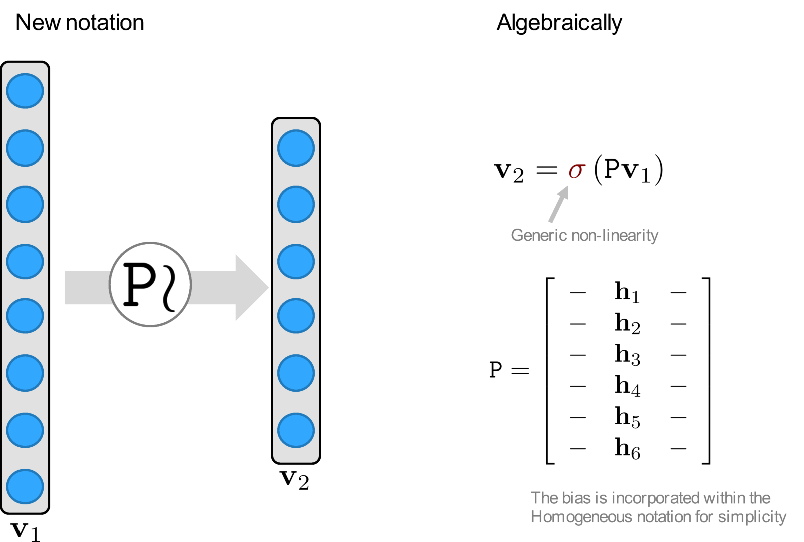
\includegraphics[width=0.7\textwidth]{projectionnotation}
   \caption{Generic projection with non-linearity, typically found in neural networks.}
   \label{fig:projectionnotation}
\end{subfigure}
~
\begin{subfigure}[b]{\textwidth}
   \centering
   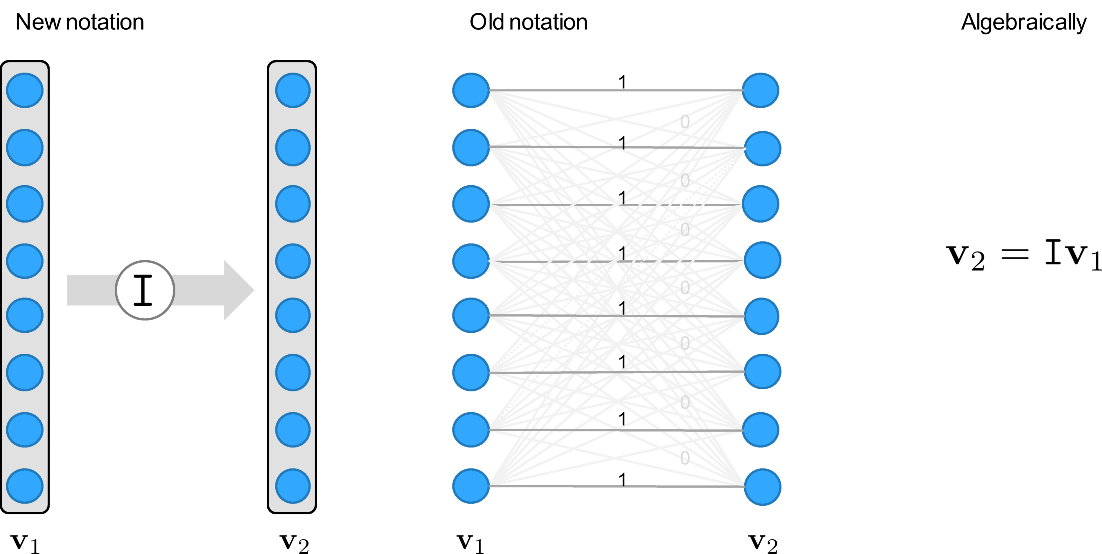
\includegraphics[width=0.9\textwidth]{identitynotation}
   \caption{Identity projection with identity function, typically found in decision trees.}
   \label{fig:identitynotation}
\end{subfigure}
~
\begin{subfigure}[b]{\textwidth}
   \centering
   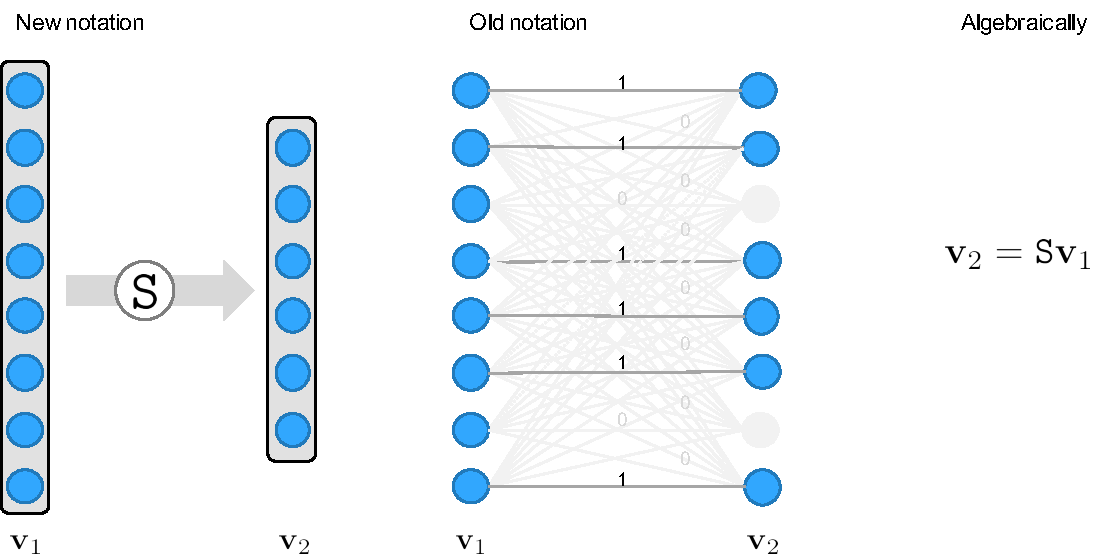
\includegraphics[width=0.9\textwidth]{selectionnotation}
   \caption{Selection projection, found in random forests.}
   \label{fig:selectionnotation}
\end{subfigure}
\caption[Various projection matrices in conditional networks.]{{\bf The proposed compact graphical notation for various types of projection in a conditional network}. \copyright Antonio Criminisi}
\label{fig:projections}
\end{figure}

This graphical language may also represent decision trees, also typically depicted in a connection-centric graphical diagram as shown in Fig.~\ref{fig:oldtreenotation}. Decision trees typically copy, or reference, samples from the root of the tree down to the leaf (or leaves) without transformation. This is notably in contrast with representation learning approaches, such as neural networks, which try to learn optimal data transformations during training with a full projection matrix, as illustrated in Fig.~\ref{fig:projectionnotation}. There have, however, been attempts to incorporate representation learning within decision forests~\cite{montillo2011entangled,BuloKontsch2014}. The copying of the sample may also be considered as a special case of the transformation $\vec v_j = \sigma(\mat P \vec v_i)$, where the projection is the identity matrix $\mat P_{ij} = \mat I$, and the function $\sigma$ is the identity function $\sigma(\vec v_i) = \vec v_i$. As such, we use the identity $\mat I$ in our graphical language to denote the routing between each tree level. This is explained graphically in Fig.~\ref{fig:identitynotation}.

Random forests consist of a number of decision trees, each of which is applied to a restricted number of the input feature dimensionality. It may not be immediately obvious how this is represented in our new graphical language, but in fact a simple extension of the above theme represents selection - \ie an identity matrix of reduced rank, as illustrated in Fig.~\ref{fig:selectionnotation}.

\subsection{Explicit Routing}
\begin{figure}[htbp!] 
\centering
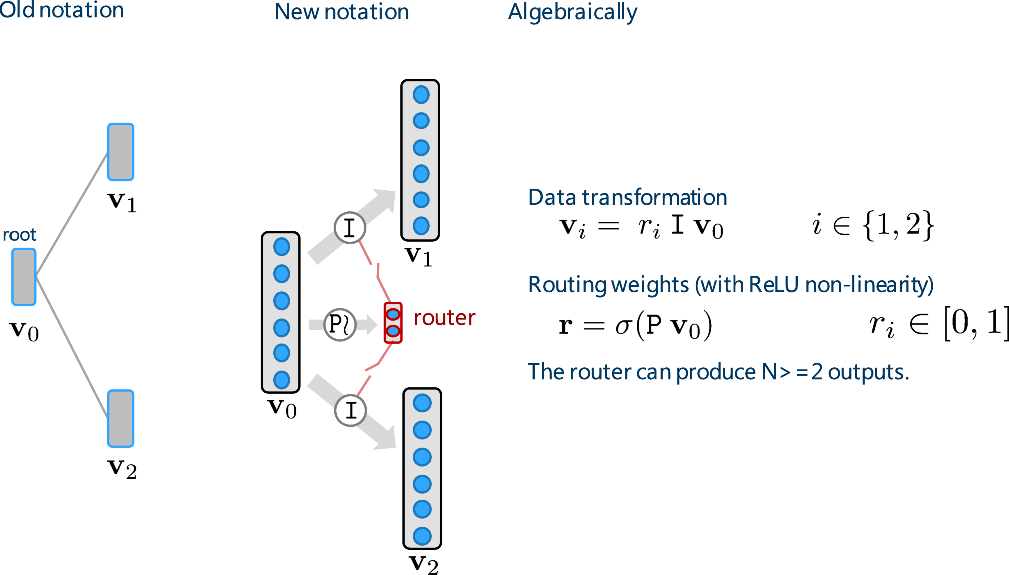
\includegraphics[width=0.95\textwidth]{treenotation}
\caption{The proposed compact graphical notation for a ``decision stump''. \copyright Antonio Criminisi}
\label{fig:treeNotation}
\end{figure}

\begin{figure}[htbp!] 
\centering
\begin{subfigure}[b]{0.4\textwidth}
   \centering
   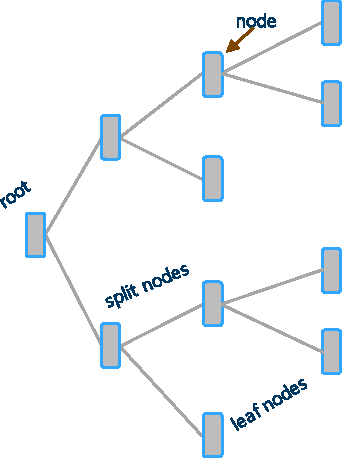
\includegraphics[width=0.95\textwidth]{oldtreenotation}
   \caption{Standard diagram of a decision tree.}
   \label{fig:oldtreenotation}
\end{subfigure}
~
\begin{subfigure}[b]{0.4\textwidth}
   \centering
   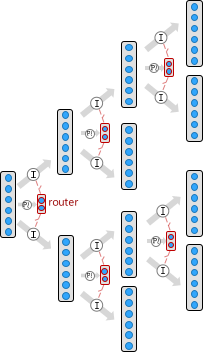
\includegraphics[width=0.8\textwidth]{newtreenotation}
   \caption{New explicit graphical notation.}
   \label{fig:newtreenotation}
\end{subfigure}
\caption{The proposed compact graphical notation for a full decision tree. \copyright Antonio Criminisi}
\label{fig:complexDecisionTree}
\end{figure}

We are still missing the method of conditional computation found in decision trees in our graphical language however, \ie how the decision is made to route each sample at a node. We must generalize two forms of routing found in decision trees, \emph{hard routing} where samples are only routed to one node in the next layer, and \emph{soft routing} where a weighted sample is potentially sent to every node of the next layer.

We achieve this with the minor addition of a new set of nodes we call a \emph{router}. A router consists of $K$ weights for a $K$-ary node or tree, as shown in Fig.~\ref{fig:treeNotation}. These router weights themselves are determined in a way more reminiscent of a neuron's activation function, typically a non-linear transformation of the sample. Thus this is represented in the same graphical notation as the mapping between neural network layers, \ie as $\mat P_{ij} \wr$. Fig.~\ref{fig:newtreenotation} shows the same tree as shown in Fig.~\ref{fig:oldtreenotation}, notably with the routers highlighted in red. Typically a router will have a number of non-zero weights and perform soft routing, however if only one of the router weights is non-zero, the router effects hard routing.


\begin{figure}[htbp!] 
\centering
\begin{subfigure}[b]{0.45\textwidth}
   \centering
   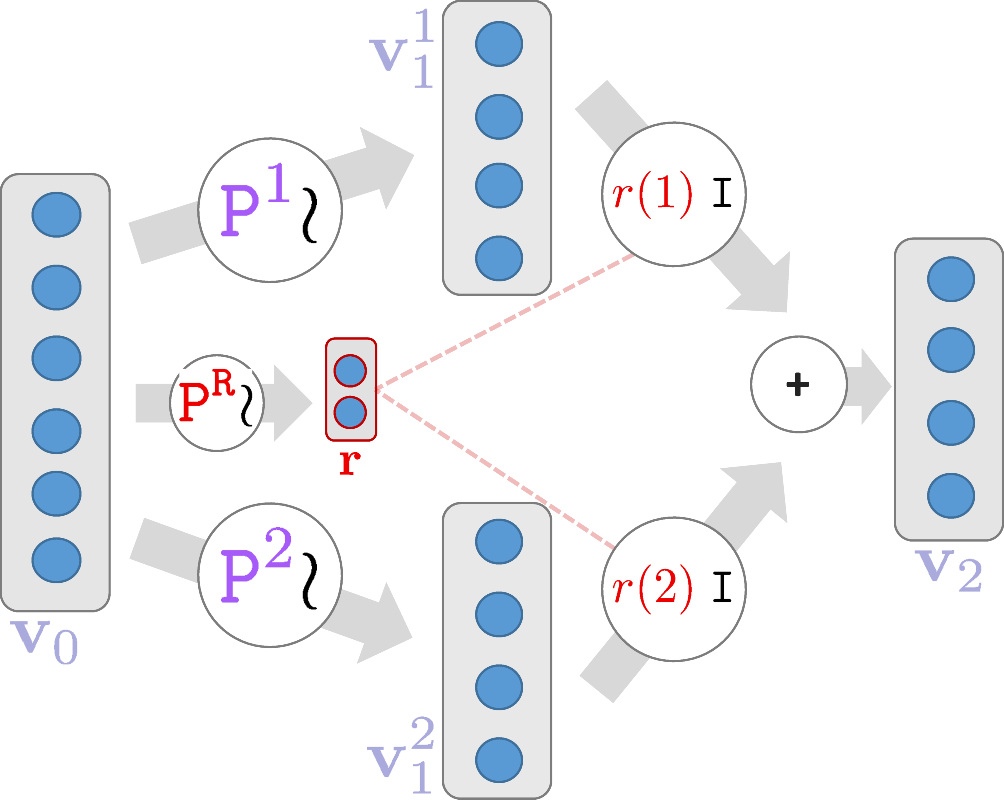
\includegraphics[width=0.95\textwidth]{explicit}
   \caption{Explicitly routed network.}
   \label{fig:explicitRouter}
\end{subfigure}
~
\begin{subfigure}[b]{0.45\textwidth}
   \centering
   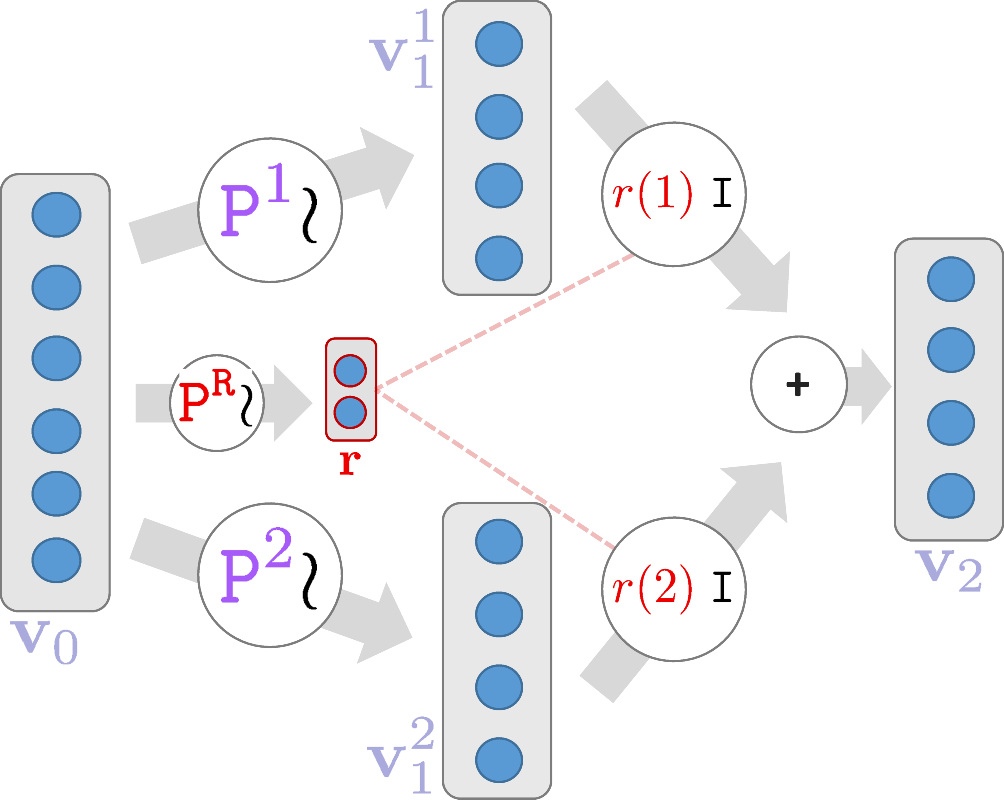
\includegraphics[width=0.95\textwidth]{explicit}
   \caption{Implcitly routed network.}
   \label{fig:implicitRouter}
\end{subfigure}
\caption{Explicit \vs Implicitly routed networks. \copyright Antonio Criminisi}
\label{fig:routerConnections}
\end{figure}

\subsection{Implicit Routing}
It is in fact possible for networks to learn a conditional routing of data without an explicit router. We call this form of conditional routing \emph{implicit routing} \vs \emph{explicit routing}, where a router is used. 

In an explicitly routed network, the routes are trained by combining the routes before the training loss. For example, in Fig.~\ref{fig:explicit} the input to layer $v_2$, $y_1$, is a linear combination of the routes weighted by the router weights, represented by $\circleplus$ operator,

\begin{equation}
	y_1 = \{y_1^j\} \forall j\circleplus \vec r = \sum_j r_j \sigma(P^j \vec v_1^j ).
\end{equation}

For an implicitly routed network instead a (non-weighted) linear combination is followed by an inner product, as used between layers of a fully connected neural network, \ie for Fig.~\ref{fig:implicit}, the input to $\vec v_2$, $y_1$,  is simply,

\begin{equation}
	y_1 = \sum_j v_1^j \sigma(P^j \vec v_0), 
\end{equation}

and hence the 

\subsection{Conditional Networks}
The generalisation, a conditional network, mixes elements of both of these models. Conditional networks may perform arbitrary projections of samples, and use arbitrary non-linear functions. Conditional networks may route samples with a soft or hard router in some or all of the layers, they may select some of all of the input feature space.

\end{document}